\documentclass[12pt, dvipdfmx]{beamer}

\renewcommand{\kanjifamilydefault}{\gtdefault}
%%%%%%%%%%%  package  %%%%%%%%%%%
\usepackage{bxdpx-beamer}% dvipdfmxなので必要
\usepackage{pxjahyper}% 日本語で'しおり'したい

\usepackage{amssymb,amsmath,ascmac}

\usepackage{multirow}
\usepackage{bm}

\graphicspath{{../../_Figures//}{../../_Figures/Rheology/}}

\usepackage{tikz}
\usepackage{xparse}

\usetikzlibrary{shapes,arrows}
%% define fancy arrow. \tikzfancyarrow[<option>]{<text>}. ex: \tikzfancyarrow[fill=red!5]{hoge}
\tikzset{arrowstyle/.style n args={2}{inner ysep=0.1ex, inner xsep=0.5em, minimum height=2em, draw=#2, fill=black!20, font=\sffamily\bfseries, single arrow, single arrow head extend=0.4em, #1,}}
\NewDocumentCommand{\tikzfancyarrow}{O{fill=black!20} O{none}  m}{
\tikz[baseline=-0.5ex]\node [arrowstyle={#1}{#2}] {#3 \mathstrut};}

%目次スライド
\AtBeginSection[]{
  \frame{\tableofcontents[currentsection]}
}

%アペンディックスのページ番号除去
\newcommand{\backupbegin}{
   \newcounter{framenumberappendix}
   \setcounter{framenumberappendix}{\value{framenumber}}
}
\newcommand{\backupend}{
   \addtocounter{framenumberappendix}{-\value{framenumber}}
   \addtocounter{framenumber}{\value{framenumberappendix}} 
}

%%%%%%%%%%%  theme  %%%%%%%%%%%
\usetheme{Copenhagen}
% \usetheme{Metropolis}
% \usetheme{CambridgeUS}
% \usetheme{Berlin}

%%%%%%%%%%%  inner theme  %%%%%%%%%%%
% \useinnertheme{default}

% %%%%%%%%%%%  outer theme  %%%%%%%%%%%
\useoutertheme{default}
% \useoutertheme{infolines}

%%%%%%%%%%%  color theme  %%%%%%%%%%%
%\usecolortheme{structure}

%%%%%%%%%%%  font theme  %%%%%%%%%%%
\usefonttheme{professionalfonts}
%\usefonttheme{default}

%%%%%%%%%%%  degree of transparency  %%%%%%%%%%%
%\setbeamercovered{transparent=30}

% \setbeamertemplate{items}[default]

%%%%%%%%%%%  numbering  %%%%%%%%%%%
% \setbeamertemplate{numbered}
\setbeamertemplate{navigation symbols}{}
\setbeamertemplate{footline}[frame number]


\title
[はじめに]
{はじめに}
\author[東亞合成 佐々木]{佐々木 裕\thanks{hiroshi\_sasaki@mail.toagosei.co.jp}}
\institute[東亞合成]{東亞合成株式会社}
\date{}

\begin{document}

%%%%%
% 1 P
%%%%%
\maketitle

%%%%%
% 2 P
%%%%%
%% 目次 (必要なければ省略)
\begin{frame}
% \frametitle{Outline}
\tableofcontents
\end{frame}

\begin{frame}
	\frametitle{ここでのお話}
		ここでは、レオロジーという「考え方」についての説明から始めていきます。
		% レオロジーを学ぶことで会社の仕事に活かせるような考え方を身に付けていただきたいと思います。
		
		この章で議論する内容について、簡単にまとめました。
		\begin{itemize}
			\item はじめに、「レオロジー」という言葉について、その歴史的背景を振り返りその流れを確認します。
			\item 次に、レオロジーが関わる分野が非常に広範囲に渡り、会社での商品開発へ有用であることを見ます。
			\item そして、人間の直感とレオロジーとの親和性が高いことについて考えてみます。
			\item 最後に、ここでの「おすすめの理解へのアプローチ」について紹介します。
		\end{itemize}
\end{frame}

\section{レオロジーとは?}
\subsection{レオロジーの始まり}
\begin{frame}
	\frametitle{レオロジーの始まり}
	\begin{columns}[T, onlytextwidth]
		\column{.6\linewidth}
		{\bf
		レオロジー (Rheology) とは、\\
		「物質の変形と流動に関する科学」
		\begin{itemize}
			\item \textit{panta rhei} (ギリシア語)
			\item ``everything flows''
			\item 万物流転
		\end{itemize}
		}
		\normalsize
		\column{.38\linewidth}
		\begin{center}
			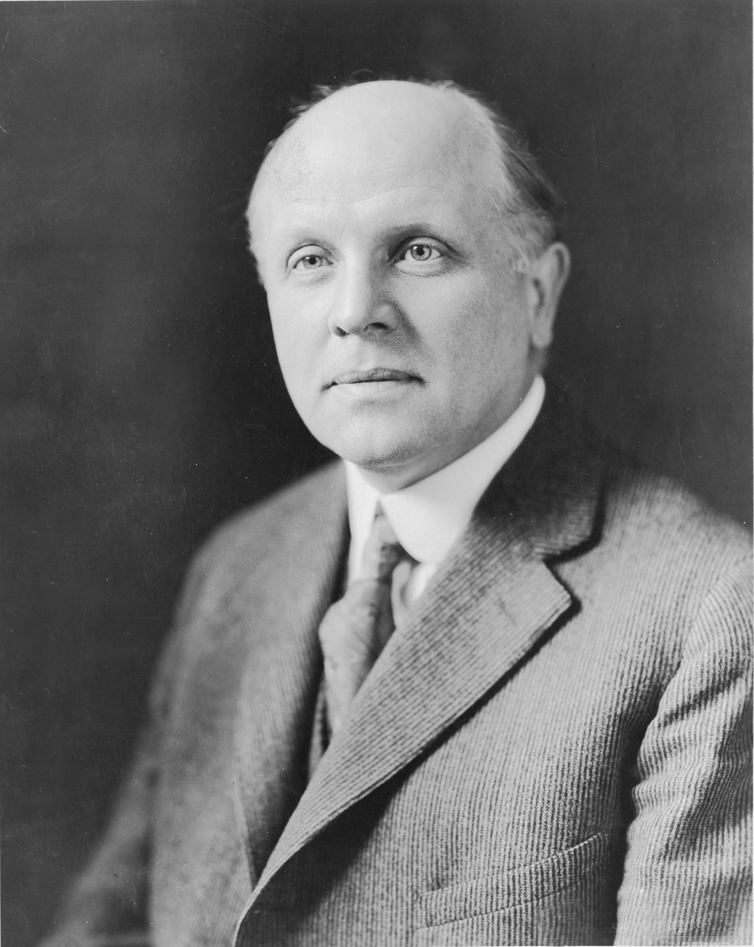
\includegraphics[width=0.6\textwidth]{Bingham.jpg}\\
			\scriptsize{\bf Eugene Cook Bingham}
		\end{center}
	\end{columns}
	\vspace{2mm}
	\small
	レオロジーという言葉は E.C. Bingham の造語であり、万物流転という意味を表すギリシア語の ``\textit{panta rhei}'' から引いた接頭語である ``Rheo-'' を学問の分野を表す ``-logy'' と組み合わせたもの。

	そして、その対象を「物質の変形と流動に関する科学」と定めたのでした。
\end{frame}

\subsection{レオロジーのやり方}
\begin{frame}
	\frametitle{古典論からレオロジーへ}
		\begin{block}{物体の変形や流動に関する古典的な物理学}
			\begin{itemize}
				\item 弾性論はフックの法則を基本にして弾性固体を対象
				\item 流体論はニュートンの法則に従う単純な流体を対象
			\end{itemize}
		\end{block}
	\begin{exampleblock}{レオロジーは}
		\begin{itemize}
			\item 弾性固体とか粘性流体のような「理想的な物体」に限らない
			「一般にそこらに存在する物質や材料」を対象に
			\item その変形と流動に関する事柄をすべて取り扱う
			\item 変形や流動というキーワード
			\item 物質や材料の特性を評価できる
			\item 工学的な考え方に有効
		\end{itemize}
	\end{exampleblock}
\end{frame}

\begin{frame}
	\frametitle{レオロジーのやり方}
	\begin{center}
		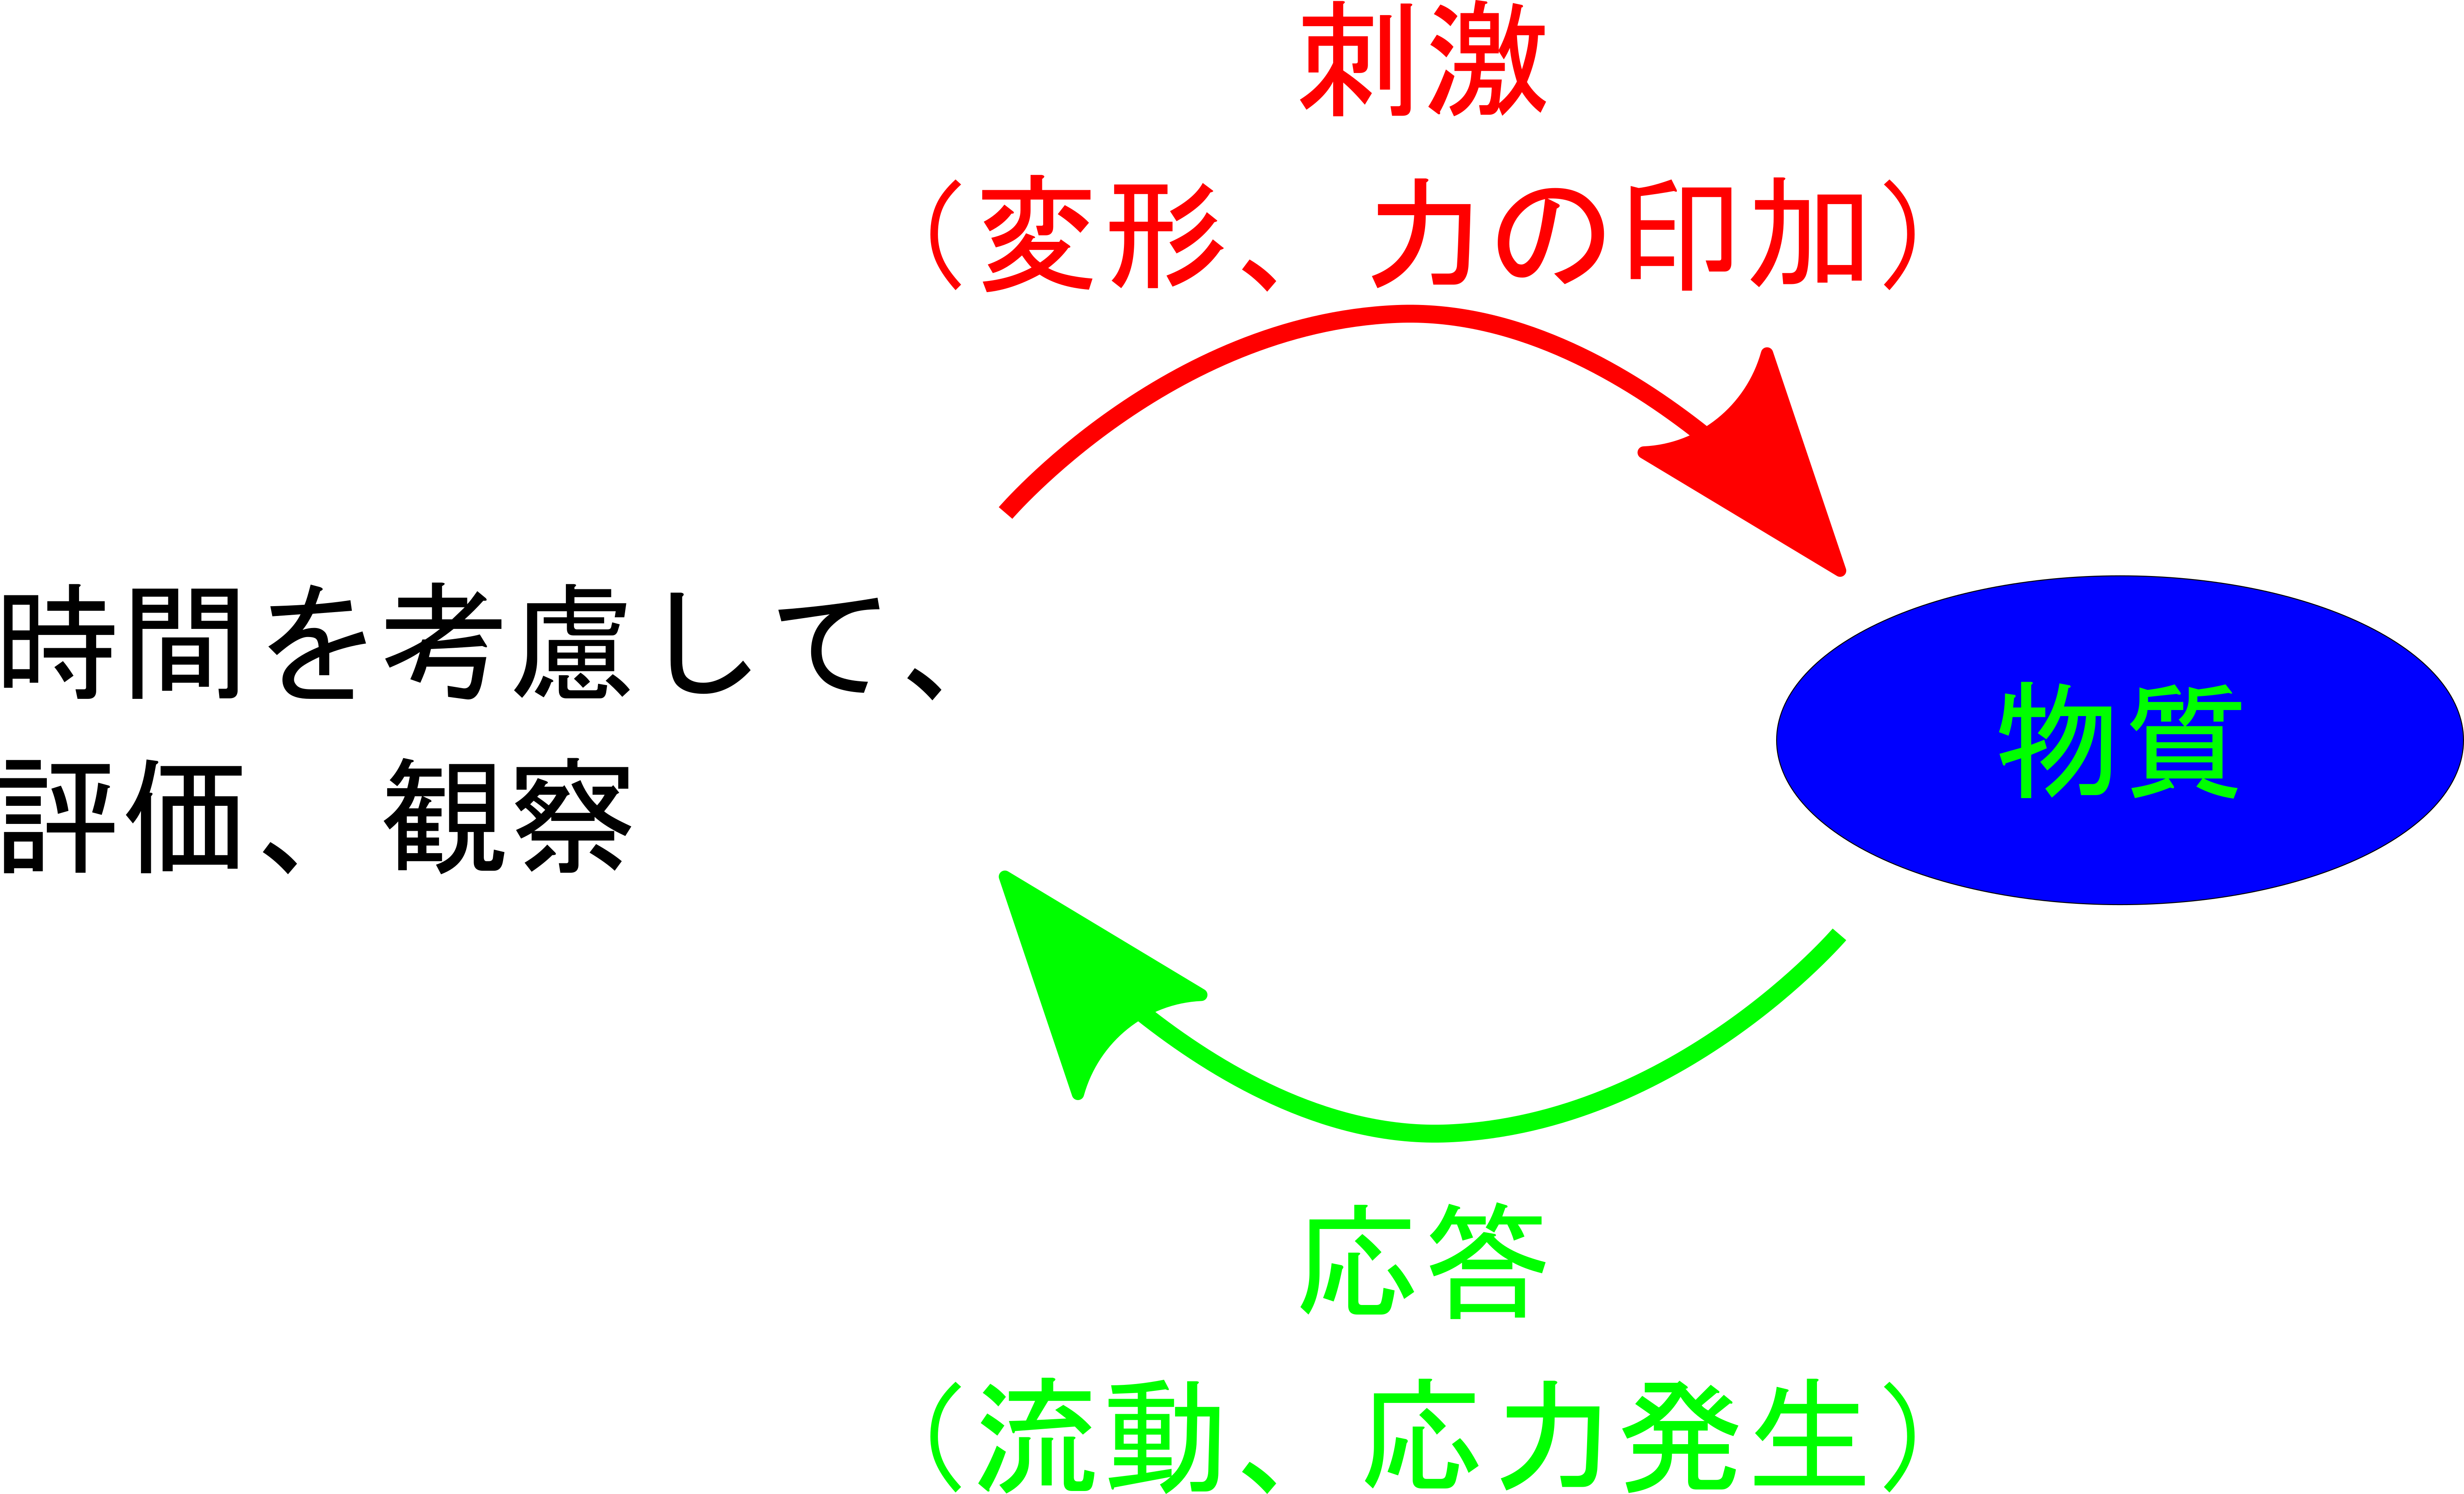
\includegraphics[width=.95\textwidth]{Rheo_method.png}
	\end{center}
\end{frame}

\section{会社の仕事とレオロジー}
\subsection{レオロジーの関わる分野}
\begin{frame}
	\frametitle{レオロジーの関わる分野}
	% 日本レオロジー学会が主催するレオロジー討論会に協賛する学会は以下のように多岐にわたる。
	\begin{block}{レオロジー討論会への協賛学会}
		日本材料学会,プラスチック成形加工学会,高分子学会,\\
		日本化学会,日本物理学会,繊維学会,応用物理学会,\\
		化学工学会,強化プラスチック協会,日本ゴム協会,\\
		日本接着学会,日本セラミックス協会,日本木材学会,\\
		セルロース学会,日本機械学会,日本雪氷学会,\\
		日本混相流学会,日本流体力学会,可視化情報学会,\\
		日本食品科学工学会,日本家政学会,日本調理科学会,\\
		日本食品工学会,日本繊維機械学会
	\end{block}
	関連分野は多岐にわたり、レオロジーは⾼度に学際的な科学と言える。
\end{frame}

\begin{frame}
	\frametitle{レオロジーの関わる分野}
	\begin{block}{学術分野としてみても幅広い}
		\begin{itemize}
			\item
			  学術分野:化学、物理、生物、化学工学、応用物理、\\
			  流体力学、地球物理学
			\item
			  高分子化学(科学):プラスチック、繊維、ゴム、\\
			  強化プラスチック
			\item
			  材料:金属、セラミックス、木材
			\item
			  応用:機械、接着、塗料、食品化学、家政学、
			  成型加工
		\end{itemize}
	\end{block}
	\begin{alertblock}{幅広い分野に渡ることで}
		\begin{itemize}
			\item 多様な切り口での議論
			\item それぞれの要素技術が異なる。
			\item 一見、複雑に見える。
		\end{itemize}
	\end{alertblock}
\end{frame}

\subsection{会社の仕事とレオロジー}
\begin{frame}
	\frametitle{会社の仕事}
	\begin{block}{開発のフローとレオロジー}	
		\begin{itemize}
			\item 会社での仕事
				\begin{itemize}
					\item 営利団体
					\item 利益を出し続けて、存続
					\item 利益を⽣み出せる商品(製品)を作りたい
				\end{itemize}
			\item 開発のフロー
				\begin{itemize}
					\item 原料⇒材料⇒商品
					\item それぞれのステップで
					\item 評価・解析に基づく、設計を⾏う。
				\end{itemize}
			\item そのステップでレオロジーも活⽤。
		\end{itemize}
	\end{block}
\end{frame}

\subsection{レオロジーと商品}
\begin{frame}
	\frametitle{商品の開発と設計}
	\begin{center}
		\includegraphics[width=\textwidth]{Katsuyou.png}
	\end{center}
\end{frame}

\begin{frame}
	\frametitle{機能設計とレオロジー}
	\begin{exampleblock}{レオロジーの活用}
		\begin{itemize}
			\item 心地良さの定量化をレオロジー的感覚で、
				\begin{itemize}
					\item 食感の定量化\\
					食品工学における「舌触り」や「のど越し」
					\item 触感の定量化\\
					肌触りの良い下着やノビの良い化粧品
				\end{itemize}
			\item 原料、材料の機能設計にレオロジーを利用
				\begin{itemize}
				\item 力学特性の評価\\
					ショックのない運動靴やよく飛ばせるゴルフクラブ
				\item 流動特性の評価\\
					塗り易くて液だれしない塗料
				\end{itemize}
		\end{itemize}
	\end{exampleblock}
\end{frame}

\section{人の感覚とレオロジー}
\subsection{人はみなレオロジスト}
\begin{frame}
	\frametitle{オノマトペとレオロジー}
	\begin{block}{オノマトペとテクスチャ}
		\begin{itemize}
			\item オノマトペとは、状態や感情を言葉に表したもの
			\item これが多彩で豊富であることが日本語の大きな特徴
			\item 織物などの手触りのような質感を表すテクスチャ
			\item 食品の食感表現にもテクスチャを表すオノマトペ
		\end{itemize}
	\end{block}
	\begin{exampleblock}{レオロジーにつながるような物性を表す言葉}
		\begin{itemize}
			\item 「サラサラは低粘度、ドロドロは高粘度」
			\item 「ふにゃふにゃは低弾性、カチカチは高弾性」
			\item フワッフワとかモッチモチ
		\end{itemize}
	\end{exampleblock}
\end{frame}

\begin{frame}
	\frametitle{人間の五感とレオロジー}
	\begin{center}
		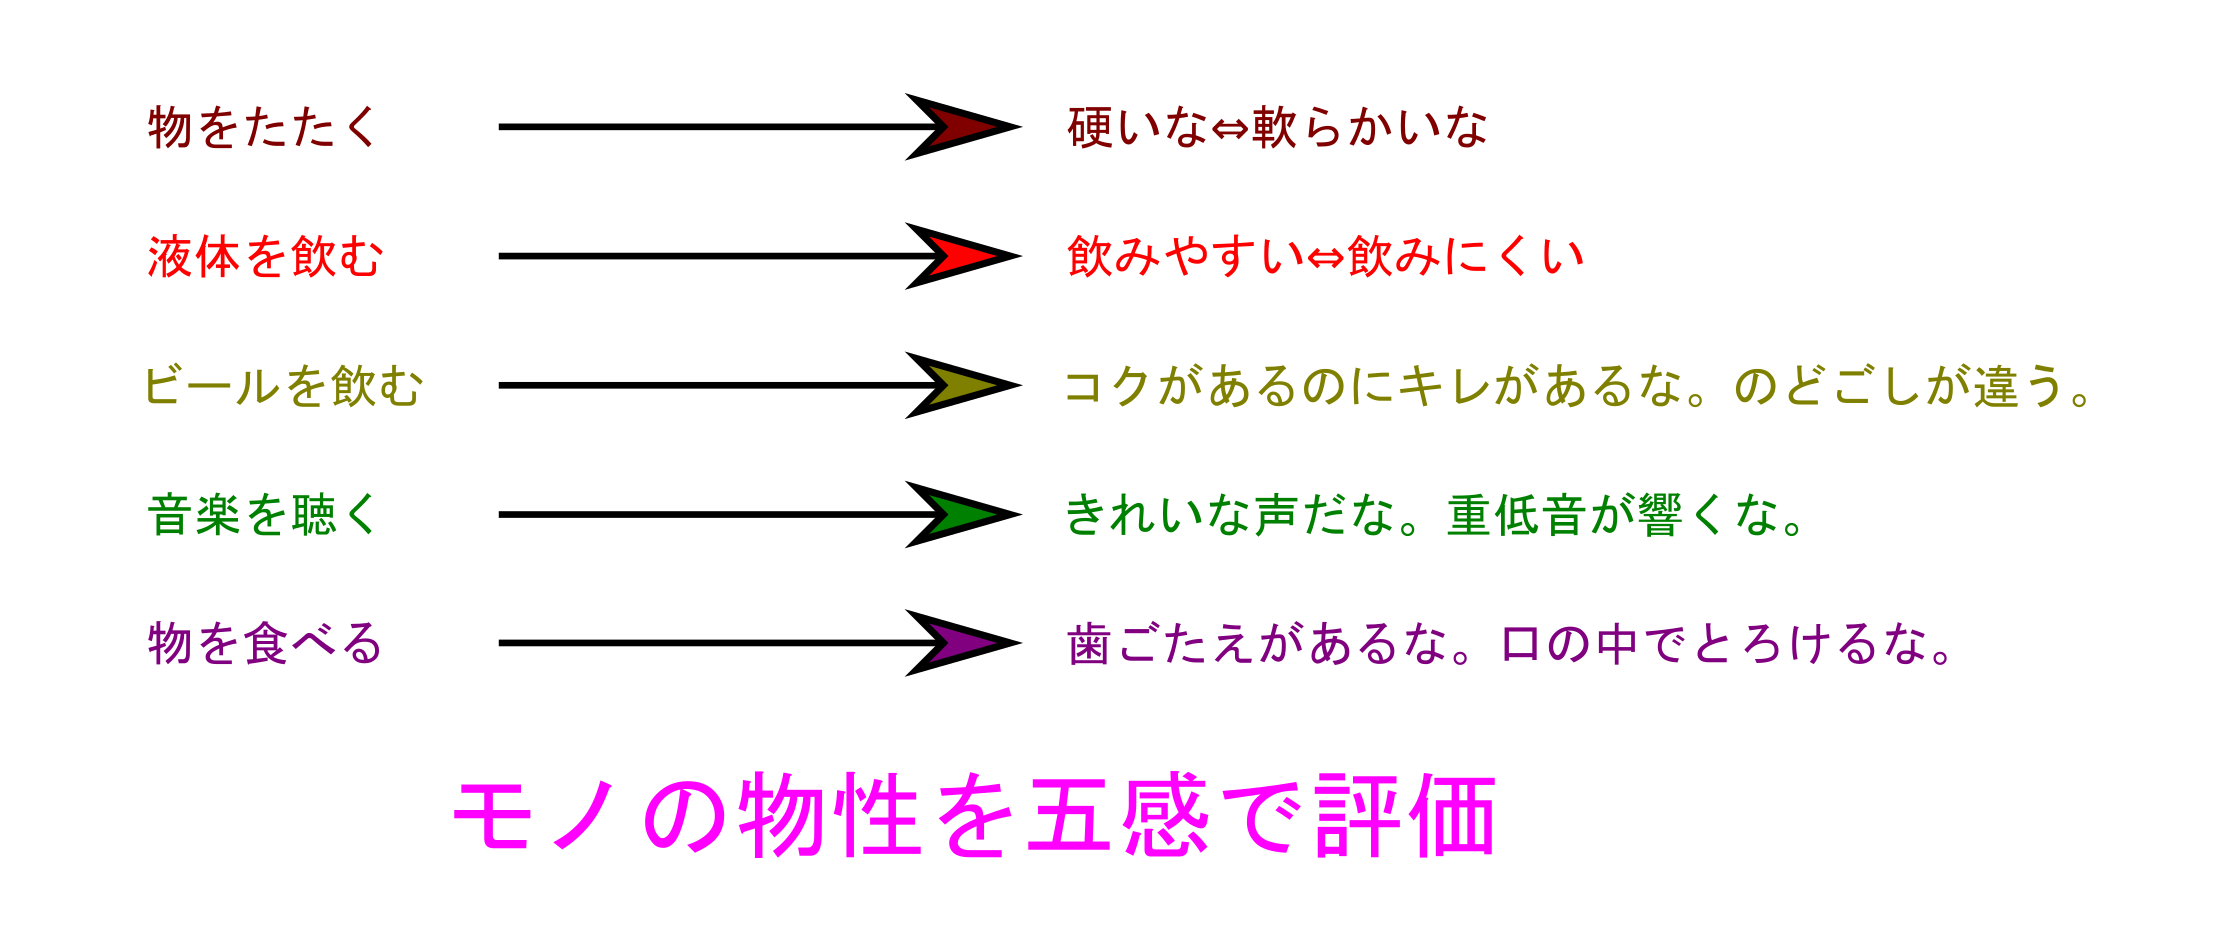
\includegraphics[width=1.1\textwidth]{gokan.png}
	\end{center}
\end{frame}

\begin{frame}
	\frametitle{人間の五感とレオロジー}
	\begin{exampleblock}{五感で評価}
		\begin{itemize}
			\item 陶磁器の品質を見分ける
			\begin{itemize}
				\item 指先ではじいてその音を聞く
				\item 焼き上がり具合に応じて振動状態が変化し、\\陶器と磁器の見分けがつく。
			\end{itemize}
			\item スイカの熟し具合
			\begin{itemize}
				\item 熟れ過ぎたスイカは音が低くなる。
				\item 実の部分に微小な気泡が生じている。
			\end{itemize}
			\item 医者が打診によって診断
			\begin{itemize}
				\item お医者さんが指で胸やお腹を叩く。
				\item 音の響きで、内臓の腫れやうっ血を判断できる。
			\end{itemize}
		\end{itemize}
	\end{exampleblock}
\end{frame}

\subsection{人間の判断基準は?}
\begin{frame}
	\frametitle{人間の判断基準は?}
		オノマトペのような言葉としての表現は感覚としての相対的な比較であり、違いを何でどのように表すかが難しい。
			\begin{block}{ウェーバー比}
				\begin{itemize}
					\item ドイツの生理学者である E. Weber は、
					% \item 様々な刺激に対する人間の感覚的な評価について、
					\item 「人間の変化を感じ取る感覚量は、受ける刺激の差ではなく何倍になったかという比に依存する」という関係
					% \item 式で表すと、
					\begin{itemize}
						\item はじめに加えられる基準となる刺激量の強度を $R$ とし、
						\item 違いに気づくことができる閾値 $\Delta R$ との間に
						\begin{align*}
							\text{ウェーバー比} = \dfrac{\Delta R}{R}= \dfrac{\text{増加量}}{\text{初期値}}
						\end{align*}
						\item そのウェーバー比は事柄ごとに決まる
					\end{itemize}
				\end{itemize}
			\end{block}
\end{frame}

\begin{frame}
	\frametitle{ウェーバー比について具体的に}
	\begin{itemize}
		% \item これを具体的に書くと、
		\item ある人が、10 の刺激が 20 になったときに「増加した」と気づくとしましょう。
		\begin{itemize}
			\item このときの増加量は、10
		\item ウェーバー比は、$\dfrac{10}{10} = 1$
		\end{itemize}
		\item その人は、20 の刺激が同じ増加量で 30 になっても、
		\begin{itemize}
			\item ウェーバー比は、$\dfrac{10}{20} = 0.5$
			\item 気づかせるためには 40 にする必要がある。
		\end{itemize}
	\end{itemize}
	\begin{alertblock}{ウェーバー比の示すこと}
		\begin{itemize}
			\item 「強い刺激を基準にすると、その違いの見分けは難しい。」
			$\Leftrightarrow$ \alert{「強い刺激には鈍感」}
			\item 人の感覚は異なるから、ウェーバー比の値も個々には異なる。
		\end{itemize}
	\end{alertblock}
\end{frame}

\begin{frame}
	\frametitle{フェヒナーの法則}
		\begin{exampleblock}{フェヒナーの法則}
			\begin{itemize}
				\item Weber の弟子である G. Fechner は、以下の対数法則
				\item 刺激の強度 $R$ が変化する時、人が感じる感覚量 $E$ は、
			\end{itemize}
			\vspace{-3mm}
			\begin{align*}
				E = C \log R \quad \text{(ここで $C$ は定数)}
			\end{align*}
		\end{exampleblock}
		\begin{block}{この数式の示すこと}
			\begin{itemize}
				\item 心理的な感覚量 $E$ は、
				\begin{itemize}
					\item 刺激の強度の値 $R$ ではなく、
					\item その対数 $\log R $ に比例して知覚される
				\end{itemize}
				\item 具体的に言えば、以下が等しいとなります。
					\begin{itemize}
						\item 100 の刺激が倍に増加して 200 になるときの感覚量
						\item 200 の刺激が倍に増加して 400 になるときの感覚量
					\end{itemize}
			\end{itemize}
			
		\end{block}
\end{frame}

\subsection{ウェーバー・フェヒナーの法則}
\begin{frame}
	\frametitle{ウェーバー・フェヒナーの法則}

	\begin{alertblock}{ウェーバー・フェヒナーの法則の意味すること}
		\begin{itemize}
			\item 刺激量の差だけではわかりにくい
			\begin{itemize}
				\item 相対変化は見やすいが、絶対的な差はわかりにくい。
			\end{itemize}
			\item 基準値によって閾値が変わる
			\begin{itemize}
				\item 元々強い刺激の変化には鈍感
				\item 基準値をそろえたほうがわかりやすい。
			\end{itemize}
			\item 差ではなく比で比較する
			\begin{itemize}
				\item 桁数の違いで感じるということが大事。
			\end{itemize}
		\end{itemize}
	\end{alertblock}
	ここで議論したような人間の感覚に関わるような分野は、心理レオロジー(サイコレオロジー)と呼ばれており、\\
	定性的な感覚量を定量化するためには重要な考え方に\\なっています。
\end{frame}

% \begin{frame}
% 	\frametitle{おまけ}
% 	\begin{itemize}
% 		\item レオロジーで何がわかるのか?
% 		\begin{itemize}
% 			\item 隠し味の調味料がわかるわけではない!
% 			\item 調味料を加えた時に、味がどう変化したのかがわかる。
% 		\end{itemize}
% 		\item 比較試料を用いて、相対値評価をする
% 		\begin{itemize}
% 			\item 絶対値評価はできない。
% 			\item 対数的な応答と考えれば、理解しやすい。
% 		\end{itemize}
% 	\end{itemize}
% \end{frame}

\section{レオロジーを理解するために}
\subsection{レオロジーの難しい点}
\begin{frame}
	\frametitle{似たものを比べると?}
	\begin{block}{身近にある水と蜂蜜を比べましょう}
		\begin{itemize}
			\item 水
				\begin{itemize}
					\item 箸で簡単にかき混ぜることができる。
					\item たやすくコップに注ぎ込むことができる。
				\end{itemize}
			\item 蜂蜜
				\begin{itemize}
					\item 容易にかき回すことができない。
					\item 入れ物を傾けても、流れにくい。
				\end{itemize}
		\end{itemize}
	\end{block}
	\begin{itemize}
		\item 触ってみたときの手応えはずいぶん違う
		\item しかしながら、その違いは感覚としての相対的な比較
		\item この違いを何で表すかが難しい
		\item 粘っこいハチミツとマヨネーズでは?
	\end{itemize}
\end{frame}

\begin{frame}
	\frametitle{言葉の使い方が曖昧}
	\begin{itemize}
		\item わかり易そうで、よくわからない表現(逃げ言葉?)\\
		以下の言葉は、レオロジーの説明によく出てきますが?
		\begin{itemize}
			\item 「応力集中が粘弾性により緩和します。」
			\item 「チクソ性の高い液体は液だれしにくい。」
			\item 「非ニュートン流体の特徴的な流動を設計しなければいけない。」
		\end{itemize}
		\item 数式の羅列で数学的なお話\\
		数式が突然天下りで出てきても!?\\
		\begin{itemize}
			\item 一般化マックスウェルモデルの動的貯蔵弾性率の数式
		\end{itemize}
	\end{itemize}
	\vspace{-4mm}
	\begin{align*}
		\displaystyle G'(\omega) = \int_{-\infty}^{\infty} \mathcal{H}(\ln \tau)\dfrac{\omega^2 \tau^2}{1 + \omega^2 \tau^2} \mathrm{d}(\ln \tau)
	\end{align*}
	\textcolor{blue}{なお、これは見た目がややこしそうというだけの例}
\end{frame}

\begin{frame}
	\frametitle{定義も不明確}
	\begin{itemize}
		\item レオロジーの対象が幅広いことも混乱しやすい原因
		\item 食感や手触りから、材料の機能性の設計に至るまで
		\item 使っている人に応じて言葉に込めた意味合いが異なる
	\end{itemize}
	\begin{exampleblock}{定義のわかりにくい例}
		\begin{itemize}
			\item 人間の心地よさをレオロジー的感覚で評価
			\begin{itemize}
				\item 「タピオカ」の喉越しのツルンとした感覚
				\item 肌触りのよい下着
			\end{itemize}
			\item 機能設計にレオロジーを利用
			\begin{itemize}
				\item ショックのない運動靴
				\item 塗り易くて液だれしない塗料
			\end{itemize}
		\end{itemize}
	\end{exampleblock}
\end{frame}

\begin{frame}
	\frametitle{よくある状態}
	\begin{exampleblock}{我々の身の回りで、よくある状態}
		\begin{itemize}
			\item ありがちな両極端
			\begin{itemize}
				\item 脳みそ筋肉状態
				\begin{itemize}
					\item 「頭で考えずに手を動かして、とにかく測れ」
				\end{itemize}
				\item 頭でっかち
				\begin{itemize}
					\item 「まずよく調べてから測定しよう」
					\item 理屈ばかりで手が動かない
				\end{itemize}
			\end{itemize}
			\item 誰もが、最初は素人 \\
			$\Leftrightarrow$ うまくやっている人の物まねが楽
			\begin{itemize}
				\item でも、近くにいい先輩がいないときは?
				\item 新しい問題へのアプローチは、誰も先輩になれない
			\end{itemize}
		\end{itemize}
	\end{exampleblock}
\end{frame}

\subsection{理解へのアプローチ}
\begin{frame}
	\frametitle{おすすめのやり方}
	{\fontsize{48pt}{10pt} \textbf{「急がば回れ」}}
	\vspace{5mm}
	\begin{alertblock}<2->{ざっくり全体像をイメージ}
		\begin{itemize}
			\item 慌てて結果を出そうとするのではなく、
			\begin{itemize}
				\item 心を落ち着けて、
				\item やるべきことを明確化してイメージ
			\end{itemize}
			\item イメージとして全体像をザックリと捕まえる
			\item 理解は一気に容易に
		\end{itemize}
	\end{alertblock}
\end{frame}

\subsection{見える化のすすめ}
\begin{frame}
	\frametitle{見える化のすすめ}
	\begin{block}{自分の中への落とし込み}
		\begin{itemize}
			\item 「何のためにやりたいのか?」を明確に。
			\begin{itemize}
				\item 目的がわからないと、ゴールが見えない。
				\item 仕事であれば、上司とよく相談。
				\item 自己啓発であれば、自分の本心をよく見極める。
			\end{itemize}
			\item 「何をやりたいのか?」を常に意識しながら、
			\begin{itemize}
				\item 因果関係をはっきりと
				\begin{itemize}
					\item 因 $\Leftarrow$ 原因
					\item 果 $\Leftarrow$ 結果
				\end{itemize}
				\item 図として捉える
				\begin{itemize}
					\item 複雑な実事象をできるだけ単純化
					\item 一目で理解できるように  
				\end{itemize}
			\end{itemize}
		\end{itemize}
	\end{block}
\end{frame}

\begin{frame}
	\frametitle{色々なモデル化}
	レオロジーという道具を理解して、何をやりたいのか?\\
	著者の場合:「様々な条件のもとで幅広い検討対象に対してでも当てはめることの出来るような、汎用的なモデル」
	\begin{exampleblock}{モデル化のすすめ}
		\begin{itemize}
			\item 適度な深さで尤もらしく
				\begin{itemize}
					\item 簡単すぎるものは例外が多い。
					\item 複雑化しすぎても過適応
						\begin{itemize}
							\item n個のデータを、n次の関数でフィット
							\item 個々の現象にだけ適応可能
							\item モデル化する意味がない
						\end{itemize}
				\end{itemize}
			\item 欲しいもの
				\begin{itemize}
					\item 汎用的に使えるモデル
					\item 尤もらしく、実験事実を説明できるもの
				\end{itemize}
		\end{itemize}
	\end{exampleblock}
\end{frame}

\begin{frame}
	\frametitle{まとめ}
		ここでは、レオロジーという「考え方」についての説明を行い、会社の仕事にどのように役立つかを考え、「おすすめの理解へのアプローチ」について紹介しました。
			\begin{block}{内容}
				\begin{itemize}
					\item 「レオロジー」という言葉の歴史的背景を振り返り、その流れを確認
					\item レオロジーが関わる分野は非常に広範囲に渡り、\\会社での商品開発に有用
					\item 人間の直感とレオロジーの親和性が高いこと
					\item 「おすすめの理解へのアプローチ」について紹介
				\end{itemize}
			\end{block}	
\end{frame}
	
% \appendix
% \backupbegin
% \section{演習問題 1}

% \subsection{「レオロジーとは?」}
% \begin{frame}
% 	\frametitle{「レオロジーとは?」}
% 	% \textcolor<2>{black}{以下の穴を埋めてください。}
% 	% \scriptsize
% 	\begin{itemize}
% 		\item \textcolor<2>{black}{レオロジー}とは、「\fbox{\textcolor<1>{white}{物質の変形と流動}}に関する科学」と呼ぶことができます。
% 		\item 物体の\fbox{\textcolor<1>{white}{変形や流動}}に関する物理学は、古くから\fbox{\textcolor<1>{white}{弾性論}}や\fbox{\textcolor<1>{white}{流体論}}として存在していました。
% 		\item 弾性論は\fbox{\textcolor<1>{white}{フックの法則}}を基本にして\fbox{\textcolor<1>{white}{弾性固体}}を記述し、流体論は\fbox{\textcolor<1>{white}{ニュートンの法則}}により粘性を持つ\fbox{\textcolor<1>{white}{単純な流体}}を対象として、それらの挙動を明確にしていました。
% 		\item レオロジーを測定する具体的な方法は、物質に\fbox{\textcolor<1>{white}{外的な刺激}}を与えて、その\fbox{\textcolor<1>{white}{応答}}としての\fbox{\textcolor<1>{white}{変形や流動}}を測ることになります。
% 		% \item 一般に、その刺激とは物質に\fbox{\textcolor<1>{white}{力学的な外力}}を与えることであり、応答としては時間という因子を意識しながら\fbox{\textcolor<1>{white}{物質のひずみ}}を測定することになります。
% 		% \item そして、このような測定を通して、物質の持つ\fbox{\textcolor<1>{white}{各種の特性}}を比較することができるようになるわけです。
% 	\end{itemize}
% \end{frame}

% \subsection{「会社の仕事とレオロジー」}
% \begin{frame}
% 	\frametitle{「会社の仕事とレオロジー」}
% 	% \textcolor<2>{black}{以下の穴を埋めてください。}
% 	% \scriptsize
% 		\begin{itemize}
% 			\item \textcolor<2>{black}{レオロジー}という学問は、高度に\fbox{\textcolor<1>{white}{学際的な科学}}であり、同時に、それぞれの\fbox{\textcolor<1>{white}{要素技術}}が大きく異る多岐にわたる対象を、\fbox{\textcolor<1>{white}{多様な切り口}}で議論していきます。
% 			\item この考え方を応用して、商品の開発の「原料から材料そして商品へと仕立てる過程」において、\fbox{\textcolor<1>{white}{特性の評価にレオロジーを活用}}することができます。
% 			\item 例えば、\fbox{\textcolor<1>{white}{人間の心地良さの定量化}}や、\fbox{\textcolor<1>{white}{原料、材料の機能設計}}にレオロジーが活用されている事例が多くあります。
% 		\end{itemize}
% \end{frame}

% \subsection{「人の感覚とレオロジー」}
% \begin{frame}
% 	\frametitle{「人の感覚とレオロジー」}
% 	% \textcolor<2>{black}{以下の穴を埋めてください。}
% 	% \scriptsize
% 		\begin{itemize}
% 			\item \textcolor<2>{black}{オノマトペ}とは\fbox{\textcolor<1>{white}{状態や感情}}を言葉に表したものであり、レオロジー的な違いを\fbox{\textcolor<1>{white}{定性的}}に表現できます。
% 			\item 人間は、ものを叩いたり触ったりして\fbox{\textcolor<1>{white}{刺激}}を与えて、その\fbox{\textcolor<1>{white}{応答}}を音で聞いたり手触りで感じることで、レオロジー評価を行う事ができます。
% 			\item 人間のレオロジー的な感覚を表現した\fbox{\textcolor<1>{white}{ウェーバー・フェヒナー}}の法則があり、基準とする値に応じて違いを見極める\fbox{\textcolor<1>{white}{閾値}}が変わるということを示しています。
% 			\item そのため、元々強い刺激の変化には鈍感で、相対変化は見やすいが、\fbox{\textcolor<1>{white}{絶対的な差}}はわかりにくいことになります。
% 		\end{itemize}
% \end{frame}

% \subsection{「レオロジーを理解するために」}
% \begin{frame}
% 	\frametitle{「レオロジーを理解するために」}
% 	% \textcolor<2>{black}{以下の穴を埋めてください。}
% 	% \scriptsize
% 		\begin{itemize}
% 			\item \textcolor<2>{black}{人間}は手触りでレオロジー的な違いを判断できますが、\fbox{\textcolor<1>{white}{定量的な}}評価を判断することはうまくできません。
% 			\item ハチミツとマヨネーズのように似たものの場合、何らかの\fbox{\textcolor<1>{white}{客観的な判断基準}}が必要となってきます。
% 			\item 感覚的な違いを言葉で表しても、その\fbox{\textcolor<1>{white}{差の大きさ}}は明確になりません。
% 			\item 著者のおすすめは、標語的には「\fbox{\textcolor<1>{white}{急がば回れ}}」であり、慌てずに、イメージとして\fbox{\textcolor<1>{white}{全体像をザックリ}}と捕まえることができれば、理解は一気に容易になります。
% 			\item 「何のためにやりたいのか」という\fbox{\textcolor<1>{white}{目的}}と「何をやりたいのか」という\fbox{\textcolor<1>{white}{目標}}をきちんと設定することが最も大事になります。
% 		\end{itemize}
% \end{frame}

% \section{演習問題 2}
% \subsection{レオロジーの使い方}
% \begin{frame}
% 	\frametitle{レオロジーの使い方}
% 	% \small
% 	「何をなんのためにやりたいのか」という目的や目標は皆さんそれぞれのものをお持ちであり、そのためにレオロジーを学ばれているのだと思います。
	
% 	この機会に、ご自身の有りたい姿について考えをまとめてみてはいかがでしょうか。
% 	\begin{itemize}
% 		\item ご自分の仕事を、全く事前の知識を持たない他の人にでも理解できるように説明してみましょう。
% 		\item ご自分の役割をシンプルに表現してみてください。
% 		\item ご自分の役割の中で、何をやらなくてはいけないと感じていますか?
% 		\item その使命は、何のためにやっているのでしょうか?
% 		\item レオロジーにはどんなことを期待していますか?
% 	\end{itemize}
% \end{frame}

% \backupend
\end{document}